\section{Empirical Evaluations}\label{sec:Results}
We now evaluate the proposed controller by deploying it to regulate the node's power while executing both training and testing applications from our use case. Later, we also compare our method with state-of-the-art controllers.

\begin{figure*}[htb]
\centering
    \vspace{-0.1cm}
    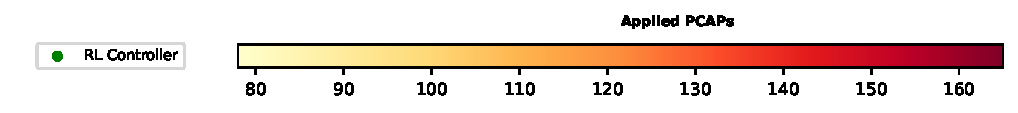
\includegraphics[width=0.8\linewidth]{Figures/legend_only.pdf} \\
    \vspace{-0.15cm}
    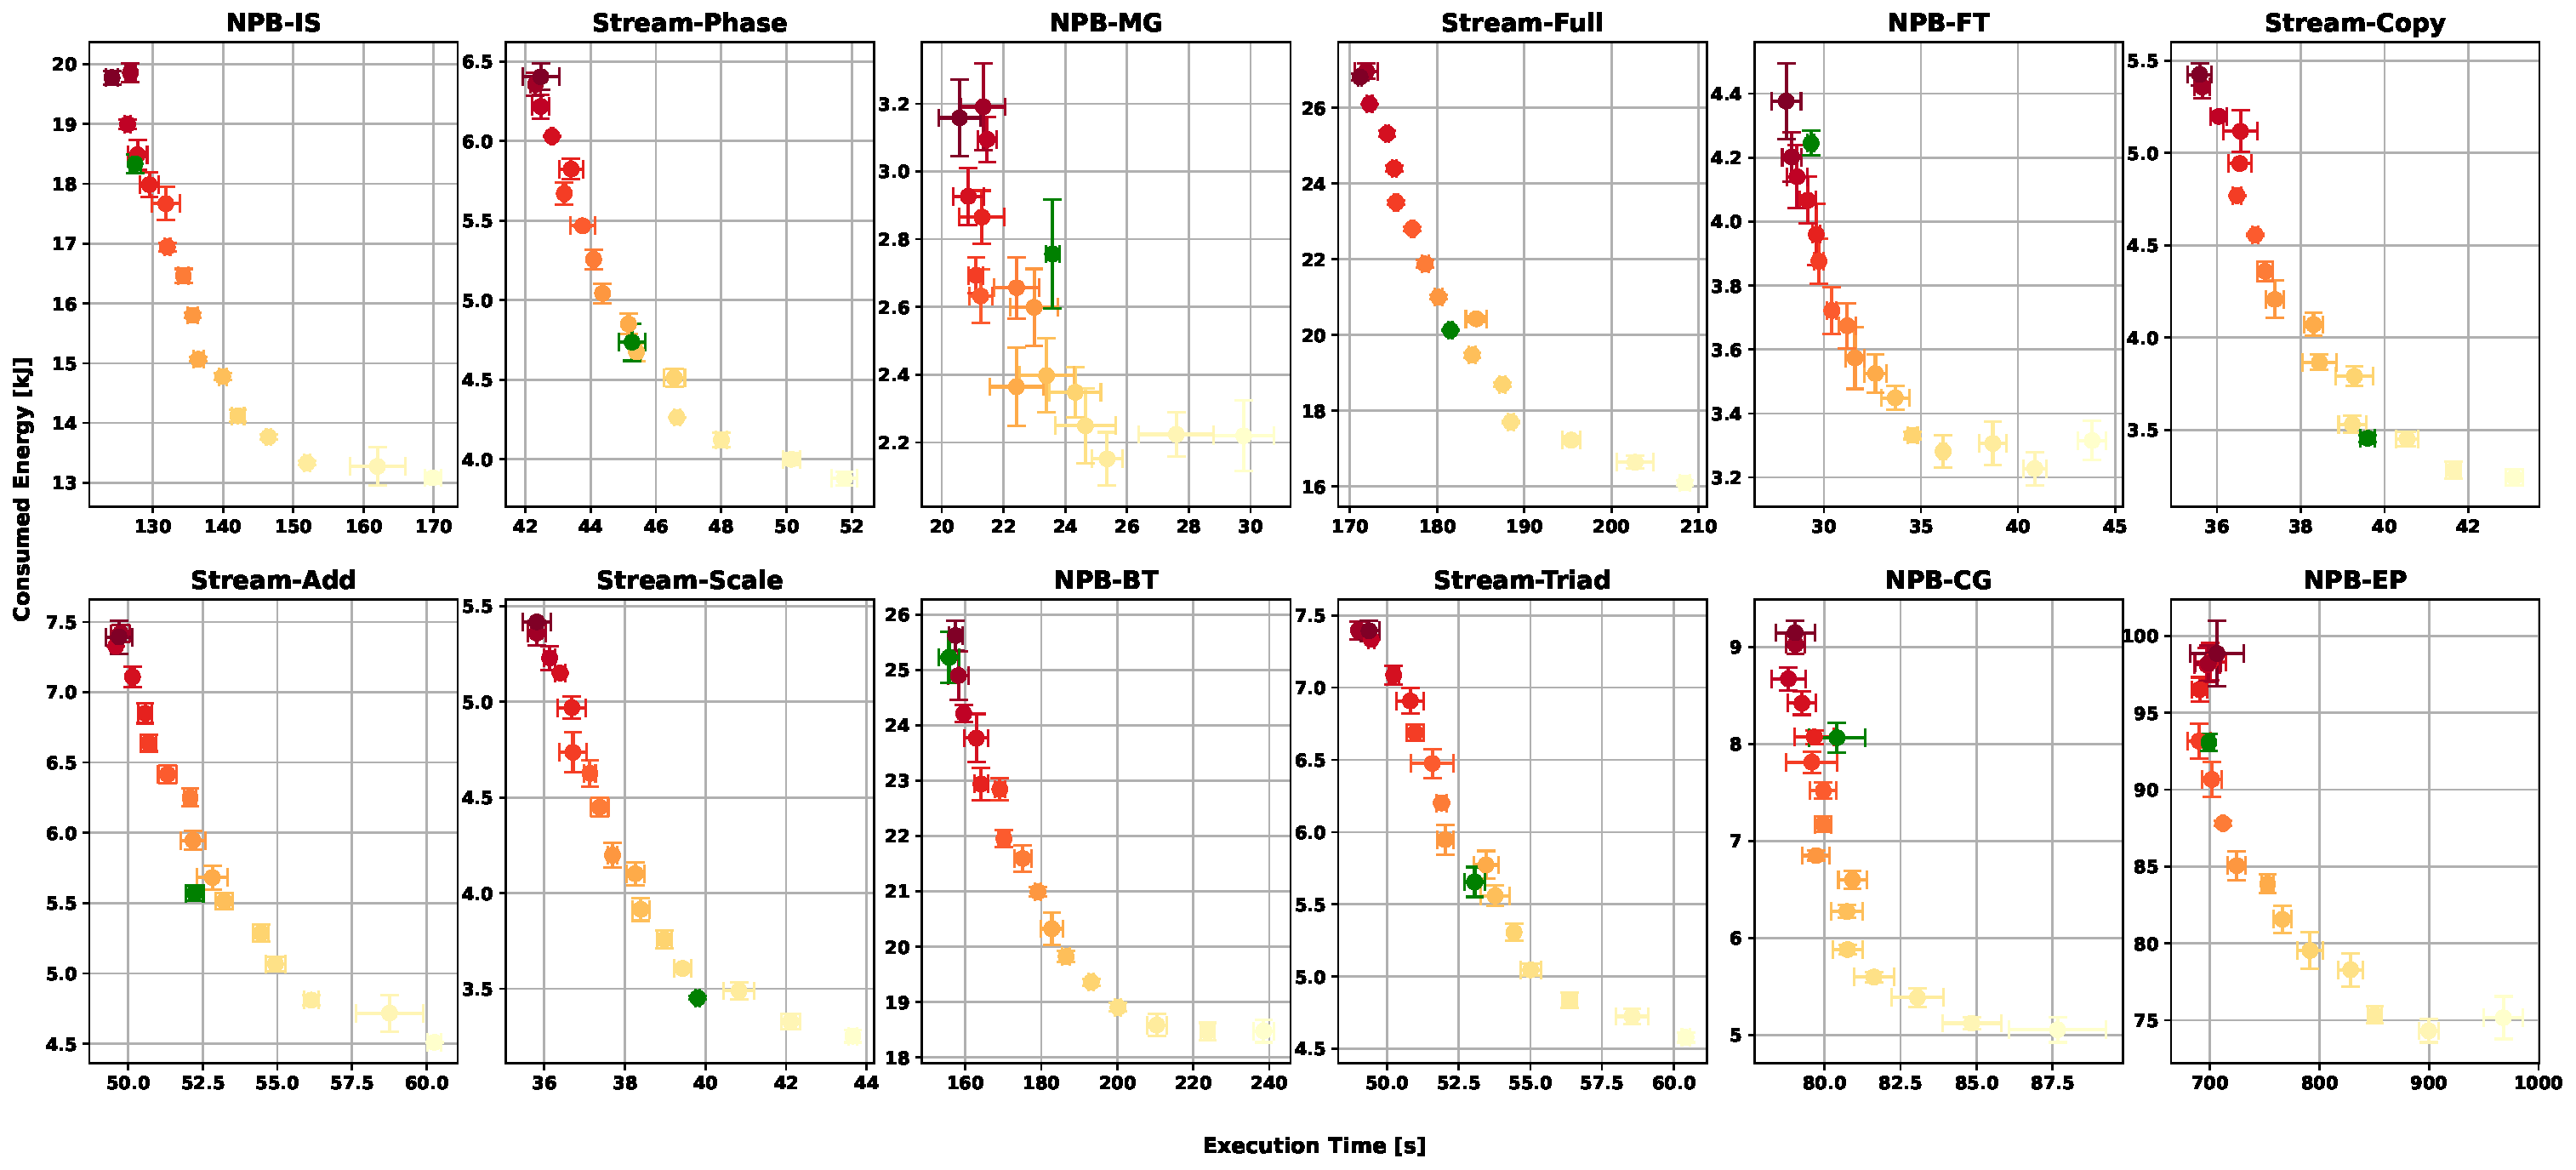
\includegraphics[width=0.95\linewidth, trim=0cm 0cm 0 0]{Figures/comparison_mean_std_dev.pdf}
    % \vspace{-0.75cm}
\caption{{Execution time vs. energy for twelve benchmarks. Six applications were unseen during training (Table \ref{tab:repeatability}). Yellow-red gradients show fixed $PCAP$ values; the green dot shows the proposed controller. Each point is averaged over five runs.}
\label{fig:comparison}}
\end{figure*}


\subsection{Evaluation of the Proposed Framework}
We assess the execution time and energy consumption in comparison with the performance of an uncapped system. In all the testing scenarios consisting of different applications, the agent evaluates states that it has never encountered during training. More out-of-distribution states are likely to appear when the proposed controller is used to regulate the power of testing applications.

For testing, we deploy our infrastructure, the trained agent, and the application together on the node of interest. The infrastructure is designed to collect the measurements ($progress$, $power$, and $PAPI$) and to provide them to the controller, which, upon postprocessing and observing the required states, makes an informed decision. The resulting action is then translated into RAPL control values and applied on the system through GEOPM.

% Akhilesh, I am not fully understanding the below setup? What exactly is happening during actual execution of test applications? Is pcap applied thruout the execution of the test appln depending on what the controller gave us? Andy, Yes, we observe and control with the RL agent being the controller deciing the power configuration (PCAP).
We first test the controller on the applications used for training, namely, the STREAM TRIAD, STREAM SCALE, NPB-IS, and NPB-EP benchmarks, which are selected to provide a large range of memory boundedness behavior. We then collect the runtime metrics and calculate the execution time and total energy consumed during the runtime for each experiment. Furthermore, we assess the performance and energy consumption of the controller with applications it has never encountered during training. For this analysis, we use the testing applications listed in Table~\ref{ch4:tab:performance_metrics}.
For comparison, we generate a Pareto curve of energy versus execution time for all the applications used in both training and testing, as shown in Figure~\ref{fig:comparison} using various static power caps. 
% Figure~\ref{fig:comparison} illustrates the relationship between energy consumption and execution time across our experiments. 

\begin{table*}[htb]
\caption{{Execution time and energy across benchmarks for Min $PCAP$, Max $PCAP$, and the proposed RL agent (mean $\pm$ std. over ten runs). RL results including energy consumed and execution time are reported relative to Max $PCAP$.}}
% \vspace{-0.5cm}
\begin{center}
\resizebox{\textwidth}{!}{%
\begin{tabular}{|c|c|c|c|c|c|c|c|c|c|c|c|c|c|c|}
\hline
\multirow{3}{*}{\textbf{Benchmark}} & \multicolumn{4}{c|}{\textbf{Min $PCAP$}} & \multicolumn{4}{c|}{\textbf{Max $PCAP$}} & \multicolumn{6}{c|}{\textbf{RL}} \\
\cline{2-15}
& \multicolumn{2}{c|}{\textbf{Execution Time}} & \multicolumn{2}{c|}{\textbf{Energy}} & \multicolumn{2}{c|}{\textbf{Execution Time}} & \multicolumn{2}{c|}{\textbf{Energy}} & \multicolumn{2}{c|}{\textbf{Execution Time}} & \multicolumn{2}{c|}{\textbf{Energy}} & \shortstack{\scriptsize{ET Degradation}  (\%)} & \shortstack{\scriptsize{Energy Saved}  (\%)} \\
\cline{2-15}
& $\mu$[\unit{s}] & $\sigma$ & $\mu$[\unit{kJ}] & $\sigma$ & $\mu$[\unit{s}] & $\sigma$ & $\mu$[\unit{kJ}] & $\sigma$ & $\mu$[\unit{s}] & $\sigma$ & $\mu$[\unit{kJ}] & $\sigma$ & (\%) & (\%) \\
\hline
\textbf{STREAM SCALE} & 37.73 & 2.61 & 4.17 & 0.61 & 34.33 & 0.47 & 5.65 & 0.08 & 37.33 & 0.47 & 3.81 & 0.05 & 8.74 & 32.61 \\
\hline
\textbf{STREAM TRIAD} & 52.86 & 3.26 & 5.83 & 0.88 & 47.67 & 0.47 & 7.67 & 0.07 & 53.67 & 0.47 & 5.15 & 0.05 & 12.59 & 32.90 \\
\hline
\textbf{NPB-EP} & 78.74 & 8.76 & 8.54 & 0.84 & 67.67 & 0.47 & 9.80 & 0.06 & 68.67 & 0.47 & 9.22 & 0.06 & 1.48 & 5.92 \\
\hline
\textbf{NPB-FT} & 37.52 & 5.81 & 4.30 & 0.35 & 30.60 & 0.49 & 5.05 & 0.08 & 31.33 & 0.47 & 4.96 & 0.08 & 2.39 & 1.78 \\
\hline
\textbf{STREAM ADD} & 53.69 & 3.88 & 5.92 & 0.86 & 48.33 & 0.47 & 7.96 & 0.08 & 55.00 & 0.82 & 5.27 & 0.08 & 13.80 & 33.74 \\
\hline
\textbf{STREAM COPY} & 38.09 & 2.92 & 4.20 & 0.60 & 34.67 & 0.47 & 5.72 & 0.08 & 37.67 & 0.47 & 3.84 & 0.05 & 8.66 & 32.91 \\
\hline
\textbf{STREAM FULL} & 189.77 & 12.24 & 20.86 & 3.13 & 172.33 & 0.47 & 28.27 & 0.07 & 183.00 & 2.52 & 20.50 & 1.22 & 6.20 & 27.47 \\
\hline
\textbf{NPB-BT} & 169.00 & 24.89 & 19.43 & 1.68 & 140.00 & 1.67 & 22.99 & 0.25 & 149.00 & 1.41 & 21.07 & 0.33 & 6.43 & 8.34 \\
\hline
\hline
\textbf{STREAM PHASES} & 93.31 & 6.26 & 10.22 & 1.52 & 84.33 & 0.47 & 13.83 & 0.07 & 94.00 & 0.00 & 9.22 & 0.01 & 11.46 & 33.34 \\
\hline
\textbf{NPB-CG} & 109.96 & 15.83 & 13.79 & 2.04 & 101.00 & 5.97 & 15.08 & 0.93 & 100.17 & 2.91 & 14.87 & 0.43 & -0.82 & 1.37 \\
\hline
\textbf{NPB-IS} & 134.85 & 11.89 & 14.67 & 1.90 & 116.67 & 1.25 & 19.17 & 0.22 & 120.67 & 0.94 & 16.88 & 0.14 & 3.43 & 11.94 \\
\hline
\textbf{NPB-MG} & 22.75 & 2.60 & 2.60 & 0.34 & 19.80 & 0.40 & 3.18 & 0.09 & 22.67 & 0.94 & 2.49 & 0.09 & 14.47 & 21.70 \\
\hline
\end{tabular}
}
\label{tab:repeatability}
\end{center}
\end{table*}

\begin{figure*}[htb]
\centering
    \vspace{-0.2cm}
    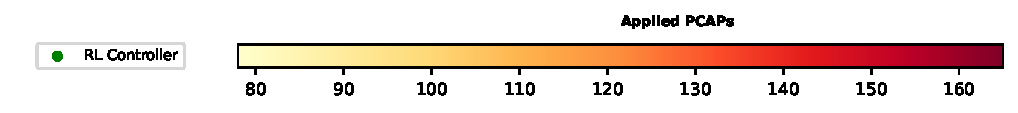
\includegraphics[width=0.8\linewidth]{Figures/legend_only.pdf} \\
    % \vspace{-0.1cm}
    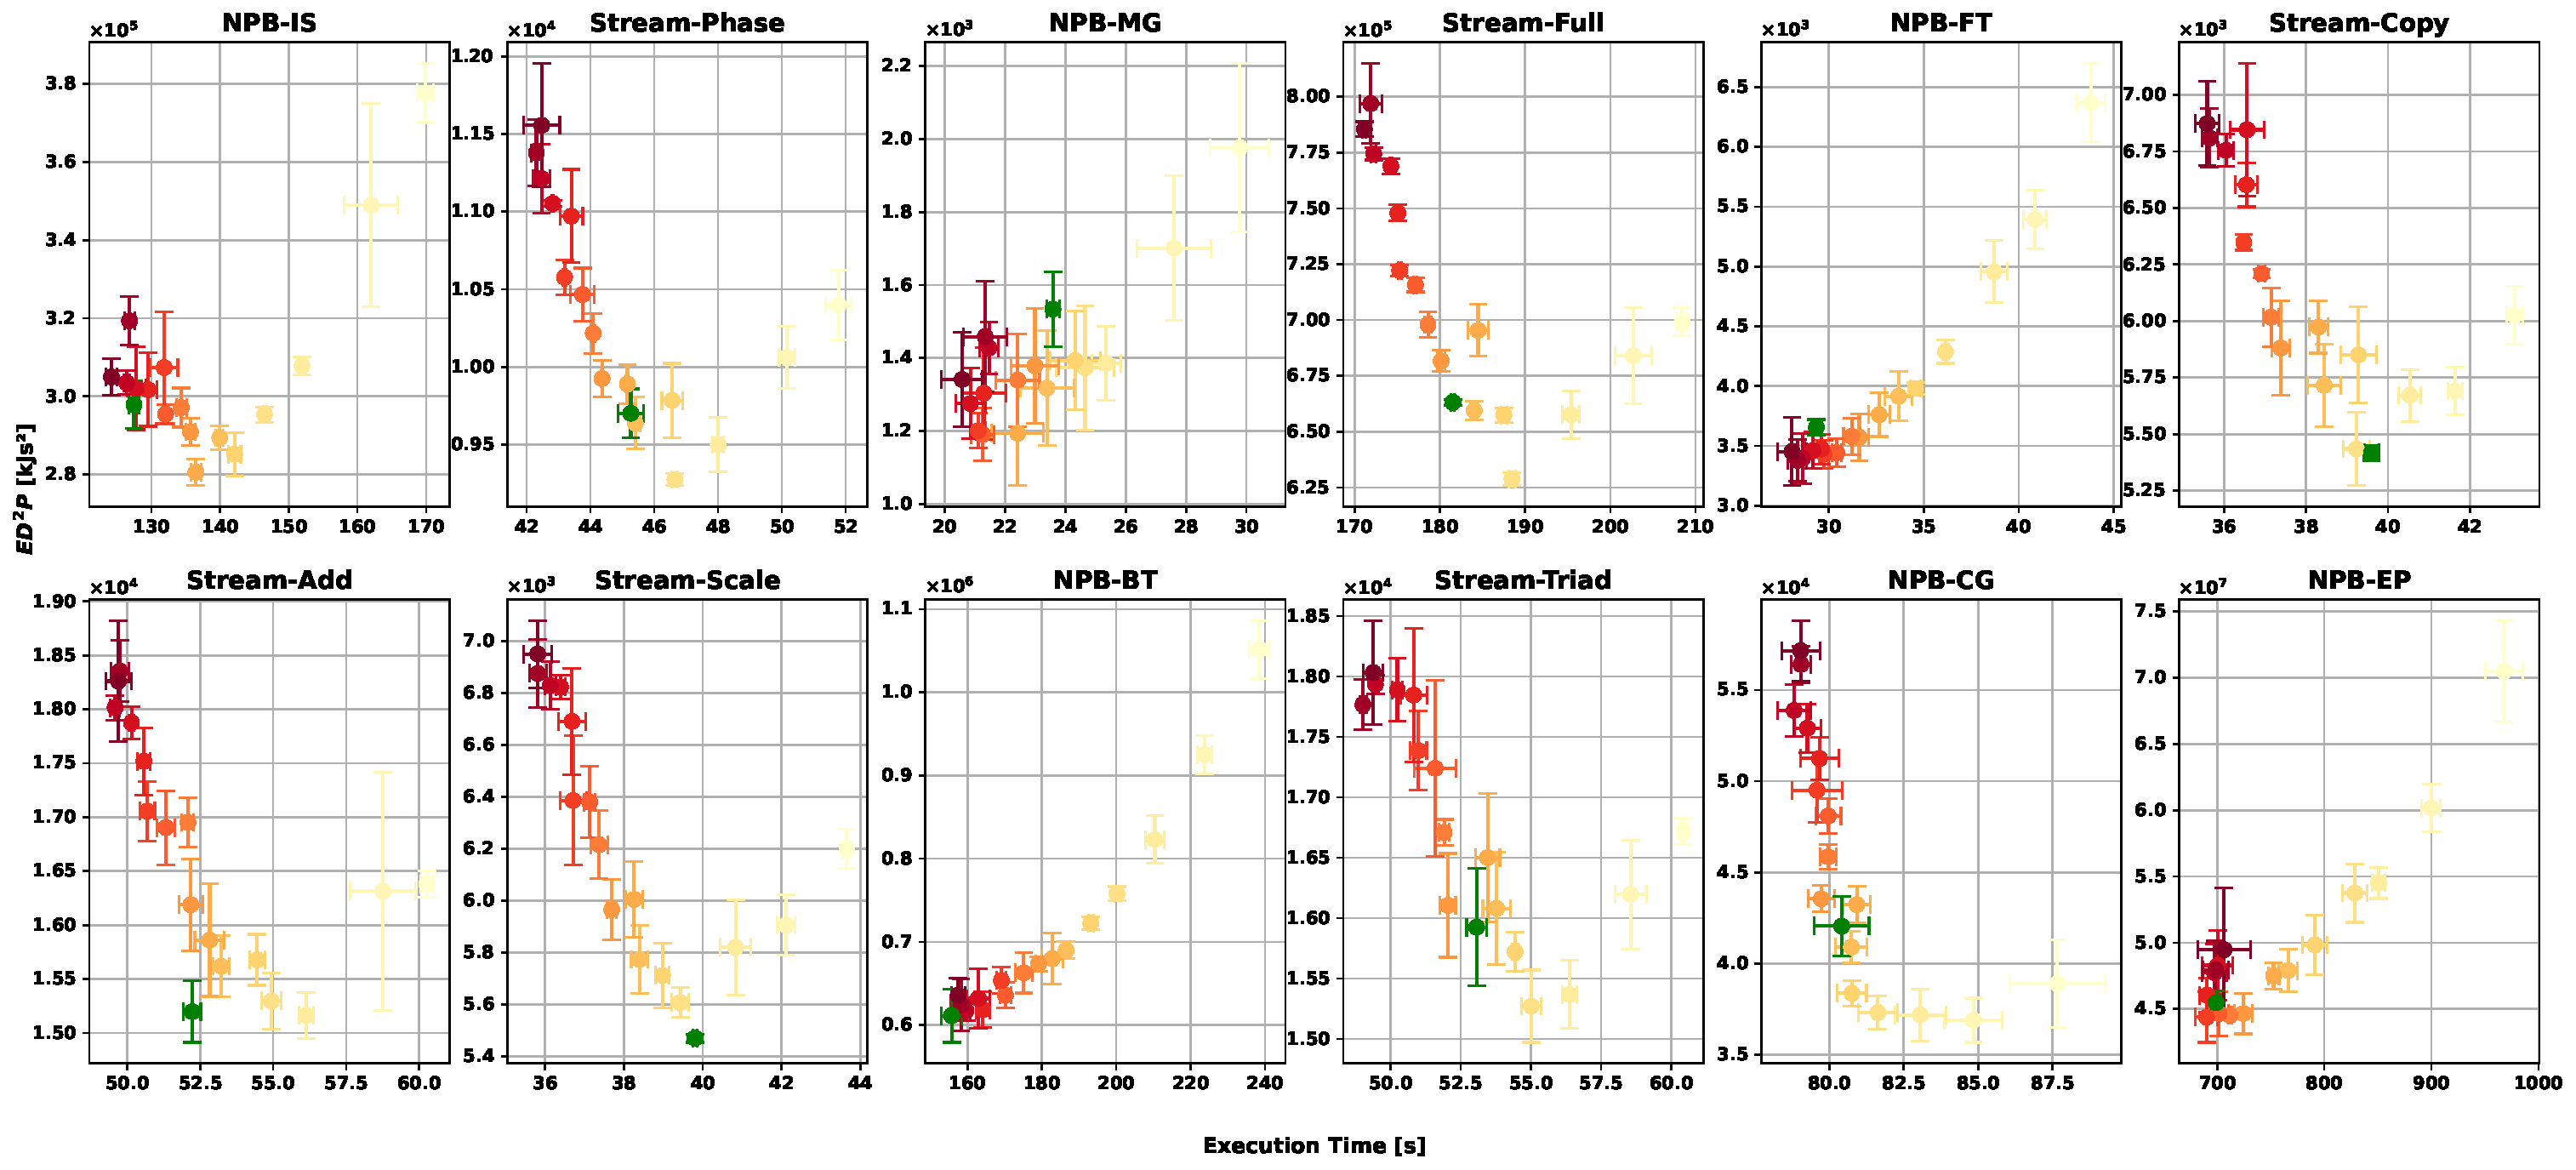
\includegraphics[width=0.95\linewidth, trim=0cm 0cm 0 0]{Figures/comparison_ED2P_mean_std_dev.pdf}
% \caption{Mean and standard deviation of $ED^2P$ scatter plots against their execution time corresponding to the experiments in \ref{fig:comparison}. It can be observed that the proposed controller was successful in keeping the average ED2P value at the lower end, irrespective of the application.}
\caption{{Mean and standard deviation of $ED^2P$ vs. execution time for the experiments in Fig.~\ref{fig:comparison}. The proposed controller consistently maintains lower average $ED^2P$ across applications.}}
\label{fig:ED2P}
%\Description{Comparison over different runs of the application.}
\end{figure*}

The comparison shows that the RL controller (green dot) consistently regulates the node's operating region between the maximum and minimum execution extremes, particularly for memory-bound applications. For compute-bound applications, the green dot typically appears on the darker end of the color bar, indicating operation under higher $PCAP$ settings. Notably, the green dot always lies on or outside the Pareto curve, demonstrating that the RL controller achieves improved or comparable performance under static workloads. This plot also highlights that the RL controller does not introduce any noticeable computational overhead on the node.

% A comparative analysis of the controlled runs versus the uncapped executions demonstrates that the RL controller consistently reduced energy usage while maintaining performance within an acceptable range of the uncapped baseline. The figure presents this data, with red gradient dots marking the finite capped runs and green dots denoting the runs under the proposed RL controller.
% The statistics for each of these runs have been tabulated under the Table~\ref{tab:repeatability}


% Figure \ref{fig:comparison} depicts the energy consumed plotted against execution time for these experiments. For the easiness of plotting and clarity, we scaled the total energy consumption and the execution time axis to a shorter span with the values of mean execution time and mean energy consumption of an uncapped system. Readers can scale up the plots, using mean values of Max $PCAP$ from Table \ref{tab:repeatability} to obtain real values.
% The controlled run of all the applications, when compared to their uncapped executions showed reduced energy consumption with negligible decay on performance. The RL-controller for all the experiments were capable of regulating the power at the maximum efficiency point. The details are given in the Figure\ref{fig:comparison} with the blue dots corresponding to finite capped runs and the purple dots corresponding to the controlled run of each application.

% To evaluate the controller's reliability, we repeated each application run ten times under three different conditions: minimum PCAP, uncapped power, and controlled PCAP. We calculated the mean execution time and energy consumption for these runs, appending this data to the initial results shown in Figure~\ref{fig:comparison}. In this figure, the green point marks the RL controller's operational regions, which consistently falls closest to the origin, indicating optimal efficiency. By computing the average performance and energy consumption across all the runs for all experiments, we assess a total energy reduction of approximately $29.07\%$ with a corresponding performance degradation of $16.05\%$.

Table~\ref{tab:repeatability} presents statistics related to the repeatability of our experiments. Together with Figure~\ref{fig:comparison}, it demonstrates that the proposed controller achieves significantly greater energy savings than any corresponding loss in performance. On average, the controller saves 20.2\% energy, with only a 7.5\%  performance decay when compared with uncapped execution.


Some exceptions can be observed in the $NPB-MG$ and $NPB-IS$ cases, which are not controlled as efficiently or as stably as the other benchmarks. We suspect that their characteristics, including a smaller average progress than most other benchmarks, might represent a challenge when not including such applications as part of the training dataset. A more exhaustive search for the ideal training set, however, becomes  prohibitively expensive as the number of applications increases. Yet, these benchmarks do not result in a performance degradation higher than that of the other benchmarks.

% These anomalies are evident from the standard deviation ($\sigma$) data in Table~\ref{tab:repeatability}, highlighting the robust yet efficient performance achieved by the RL controller under varying conditions. We can always improve these results with fine tuning of the hyper parameters and better post processing of the data. The shortened sampling intervals between the sensing for observation and actuation has also caused the noisy measurements.



% To analyze the stability of the controller in repeatability of the experiments, we ran the applications 10 different times, repeated under minimum $PCAP$ (lowest $PCAP$ supported by $RAPL$), uncapped power and the controlled $PCAP$. We calculated the mean values of their execution time and energy consumption, and added it alongside the initial results shown in Figure \ref{fig:comparison}. The point in red corresponds to the mean operating region of the $RL$ controller which is closest to the origin in all the cases. Similarly the green and orange points correspond to the lowest $PCAP$ and uncapped executions respectively. The statistics of the executions are given in Table\ref{tab:repeatability}. Referring to Figure \ref{fig:comparison} and Table \ref{tab:repeatability} one can observe the percentage reduction in the energy consumption is more than the percentage degradation in performance when compared to the uncapped runs of all the applications. 
% Due to the presence of outliers in some of the $ones-stream-full$ and $ones-npb-EP$ executions, performance degradation was not observed in these cases, even with reduced energy consumption. These facts can be verified from Table \ref{tab:repeatability} from the standard deviation ($\sigma$) column.
% \begin{figure*}[htb]
% \centering
%     \vspace{-0.1cm}
%     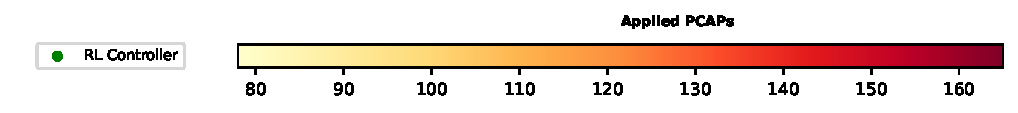
\includegraphics[width=0.9\linewidth]{Figures/legend_only.pdf} \\
%     \vspace{-0.3cm}
%     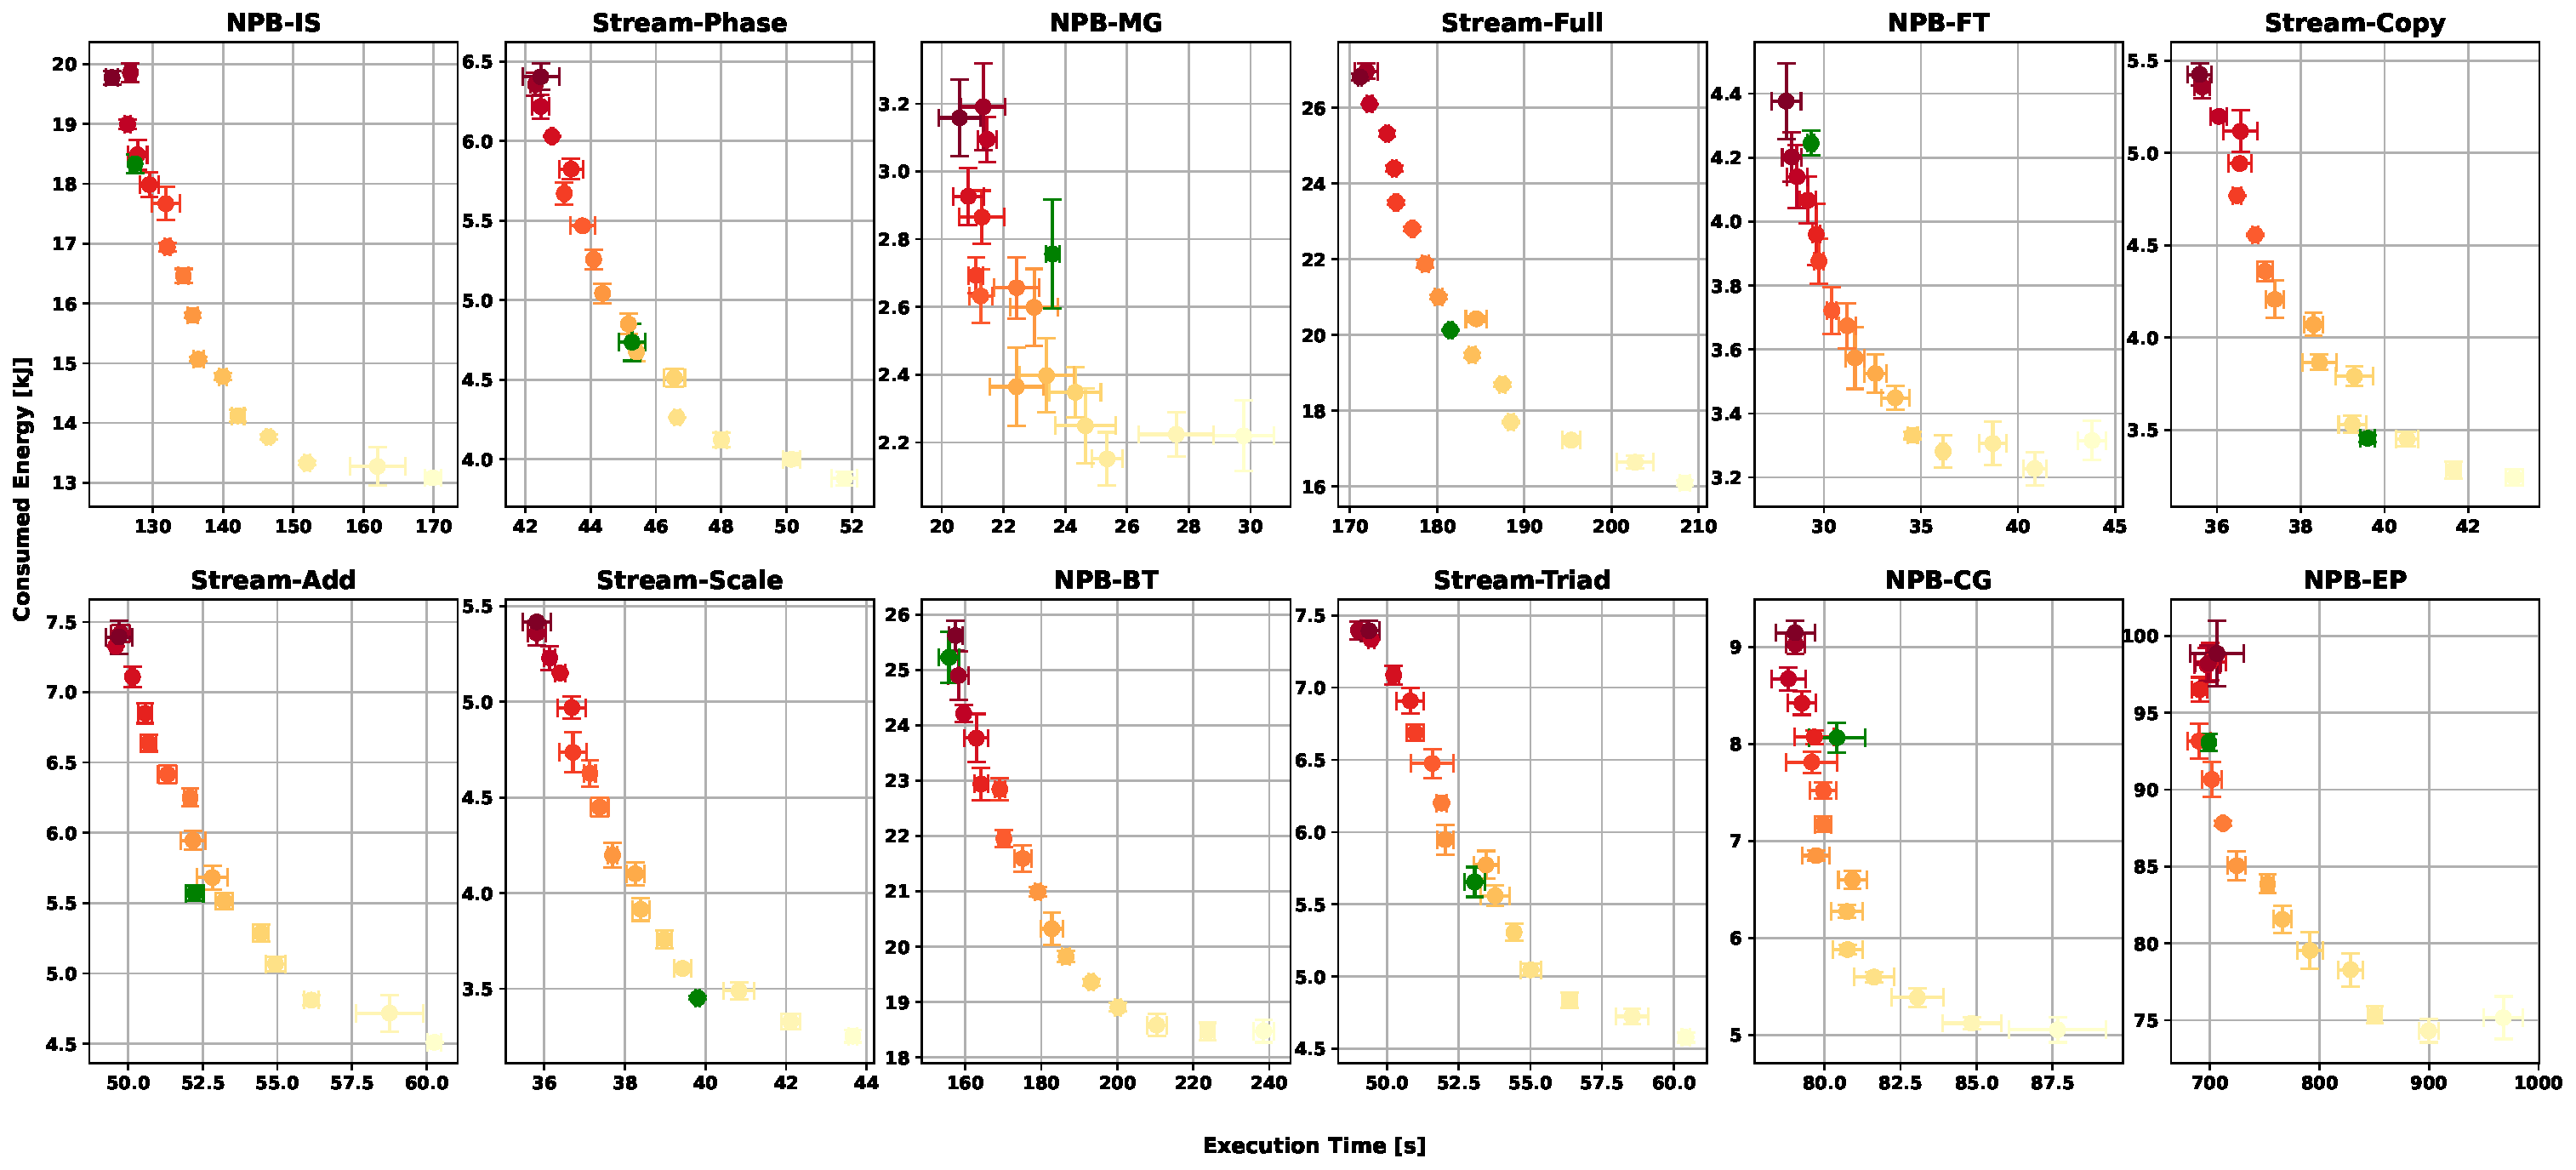
\includegraphics[width=\linewidth, trim=0cm 0cm 0 0]{Figures/comparison_mean_std_dev.pdf}
%     \vspace{-0.75cm}
% % \caption{Execution time versus energy scatter plots for the evaluation of eight benchmark applications. Among these, four applications were not included in the training set. The yellow - red gradients represent executions under a constant $PCAP$ while the green dot indicates results under the proposed controller. Each of these points correspond to the average over 5 executions of each of the experiments.  The scales are normalized against their maximum values for better readability.}
% \caption{Execution time vs. energy for ten benchmarks. Six applications were unseen during training (Table \ref{tab:repeatability}). Yellow-red gradients show fixed $PCAP$ values; the green dot shows the proposed controller. Each point is averaged over five runs.}
% \label{fig:comparison}
% %\Description{Comparison over different runs of the application.}
% \end{figure*}


To understand the impact of the proposed controller in optimizing the target objective, we plot the $ED^2P$ values corresponding to each of these experiments. The results appear in Figure~\ref{fig:ED2P}. 


The results show that the proposed controller was able to regulate power across different application scenarios, often where the $ED^2P$ value was close to its global minimum. Compared with the uncapped power setting, the controller gave better results in all cases.
% Since there is no known optimal closed-loop controller, it is useful to compare against the uncapped case.

% \vspace{-0.2cm}
% For an effective evaluation of the controller in diverse performance scenarios, it is crucial to test its functionality during the variable phases of an application's runtime.
% We also analyzed the controller's adaptability to these fluctuations by utilizing a STREAM application that executes different kernels iteratively. We selected the $Stream-Phases$ application, with all four kernels running 500 times in a cycle repeated over 5 iterations. 

\sisetup{
  scientific-notation=true,
  round-mode=figures,
  round-precision=3,
  detect-weight=true,
  detect-inline-weight=math
}
\newcommand{\bestg}[1]{\cellcolor{green!25}\textbf{#1}}
\newcommand{\worstr}[1]{\cellcolor{red!15}#1}

\begin{table*}[t]
\begin{center}
\resizebox{\textwidth}{!}{%
\begin{tabular}{|c|ccc|ccc|ccc|ccc|ccc|}
\hline
\multirow{3}{*}{\textbf{Benchmark}} &
\multicolumn{3}{c|}{\textbf{DVFS Controller}} &
\multicolumn{3}{c|}{\textbf{PI-Global Model}} &
\multicolumn{3}{c|}{\textbf{PI-App-Specific Model}} &
\multicolumn{3}{c|}{\textbf{Ondemand Governor}} &
\multicolumn{3}{c|}{\textbf{RL (Ours)}} \\
\cline{2-16}
& \shortstack{\scriptsize Energy\\Saved (\%)} &
  \shortstack{\scriptsize Perf\\Degrad. (\%)} & \textbf{ED$^{2}$P} &
  \shortstack{\scriptsize Energy\\Saved (\%)} &
  \shortstack{\scriptsize Perf\\Degrad. (\%)} & \textbf{ED$^{2}$P} &
  \shortstack{\scriptsize Energy\\Saved (\%)} &
  \shortstack{\scriptsize Perf\\Degrad. (\%)} & \textbf{ED$^{2}$P} &
  \shortstack{\scriptsize Energy\\Saved (\%)} &
  \shortstack{\scriptsize Perf\\Degrad. (\%)} & \textbf{ED$^{2}$P} &
  \shortstack{\scriptsize Energy\\Saved (\%)} &
  \shortstack{\scriptsize Perf\\Degrad. (\%)} & \textbf{ED$^{2}$P} \\
\cline{2-16}
&  &  &  &  &  &  &  &  &  &  &  &  &  &  &  \\
\hline

\textbf{NPB-BT} &
\worstr{-13.50} & \worstr{13.90} & \worstr{\num{6.63436e5}} &
\worstr{-98.43} & \bestg{-0.21} & \num{8.90421e5} &
-5.12 & 7.14 & \num{5.43782e5} &
-13.50 & 13.90 & \num{6.63436e5} &
\bestg{8.34} & 6.43 & \bestg{\num{4.67824e5}} \\
\hline

\textbf{NPB-CG} &
-7.74 & -1.44 & \num{1.60989e5} &
\worstr{-13.56} & \worstr{9.57} & \worstr{\num{2.09714e5}} &
2.23 & 0.99 & \num{1.53389e5} &
-11.47 & 11.17 & \num{2.11919e5} &
\bestg{1.37} & \bestg{-0.83} & \bestg{\num{1.49226e5}} \\
\hline

\textbf{NPB-EP} &
-0.80 & -1.56 & \num{4.38312e4} &
\worstr{-124.00} & \worstr{16.87} & \worstr{\num{1.37298e5}} &
6.33 & 4.43 & \num{4.58408e4} &
-9.97 & 15.63 & \num{6.59907e4} &
\bestg{5.93} & \bestg{1.47} & \bestg{\num{4.34663e4}} \\
\hline

\textbf{NPB-FT} &
-5.70 & \worstr{36.42} & \num{9.30167e3} &
\worstr{-123.59} & 16.31 & \num{1.43021e4} &
0.02 & 13.07 & \num{6.04468e3} &
\bestg{10.51} & \bestg{4.65} & \bestg{\num{4.63399e3}} &
1.78 & 2.40 & \num{4.86997e3} \\
\hline

\textbf{NPB-IS} &
-8.17 & \worstr{23.42} & \num{4.29962e5} &
\worstr{-127.69} & 17.41 & \worstr{\num{8.18978e5}} &
10.45 & 4.28 & \num{2.54109e5} &
-5.54 & 7.65 & \num{3.19145e5} &
\bestg{11.96} & \bestg{3.43} & \bestg{\num{2.45745e5}} \\
\hline

\textbf{NPB-MG} &
-11.04 & 27.19 & \num{2.23950e3} &
\worstr{-162.41} & \worstr{33.39} & \worstr{\num{5.82111e3}} &
6.23 & \bestg{-1.32} & \bestg{\num{1.13841e3}} &
-12.72 & 15.20 & \num{1.86513e3} &
\bestg{21.79} & 14.48 & \num{1.27779e3} \\
\hline

\textbf{STREAM FULL} &
7.76 & 1.50 & \num{7.97888e5} &
\worstr{-47.49} & \worstr{19.33} & \worstr{\num{1.76332e6}} &
9.21 & 4.06 & \num{8.25458e5} &
1.23 & 0.29 & \num{8.34002e5} &
\bestg{27.50} & \bestg{6.19} & \bestg{\num{6.86421e5}} \\
\hline

\textbf{STREAM TRIAD} &
7.66 & 12.86 & \num{2.05003e4} &
\worstr{-128.48} & \worstr{20.24} & \worstr{\num{5.75778e4}} &
11.17 & 10.48 & \num{1.88981e4} &
-4.44 & \bestg{6.45} & \num{2.06296e4} &
\bestg{32.82} & 12.58 & \bestg{\num{1.48407e4}} \\
\hline

\textbf{STREAM ADD} &
10.97 & 13.96 & \num{2.14976e4} &
\worstr{-147.56} & \worstr{27.35} & \worstr{\num{7.46519e4}} &
\bestg{35.17} & \bestg{4.60} & \bestg{\num{1.31873e4}} &
0.60 & 2.87 & \num{1.95567e4} &
33.77 & 13.80 & \num{1.59476e4} \\
\hline

\textbf{STREAM SCALE} &
9.61 & 15.77 & \num{8.06690e3} &
\worstr{-131.15} & \worstr{22.24} & \worstr{\num{2.29990e4}} &
12.17 & 8.75 & \num{6.91671e3} &
-0.84 & \bestg{6.49} & \num{7.61543e3} &
\bestg{32.65} & 8.75 & \bestg{\num{5.30353e3}} \\
\hline

\textbf{STREAM COPY} &
5.63 & 16.86 & \num{8.86046e3} &
\worstr{-143.02} & \worstr{28.76} & \worstr{\num{2.77001e4}} &
11.65 & 11.53 & \num{7.55612e3} &
1.23 & \bestg{4.82} & \num{7.46148e3} &
\bestg{32.83} & 8.64 & \bestg{\num{5.45115e3}} \\
\hline

\textbf{STREAM PHASES} &
11.15 & 14.51 & \num{1.14581e5} &
\worstr{-65.80} & \worstr{24.02} & \worstr{\num{2.50832e5}} &
2.20 & 7.12 & \num{1.10376e5} &
-0.35 & \bestg{3.38} & \num{1.05472e5} &
\bestg{33.35} & 11.47 & \bestg{\num{8.14447e4}} \\
\hline\hline

\textbf{Average} &
0.49 & 14.45 & \num{1.90096e5} &
\worstr{-109.43} & \worstr{19.61} & \worstr{\num{3.56135e5}} &
8.48 & 6.26 & \num{1.65558e5} &
-3.77 & 7.71 & \num{1.88477e5} &
\bestg{20.34} & \bestg{7.40} & \bestg{\num{1.43485e5}} \\
\hline
\end{tabular}
}
\caption{{Controllers compared with uncapped (Max PCAP). Only rowwise extremes are colored: \textbf{green} = best (max Energy Saved, min Perf Degradation, min ED$^{2}$P); \textbf{red} = worst (min Energy Saved, max Perf Degradation, max ED$^{2}$P). Lower ED$^{2}$P is better.}}
\label{tab:controllers_vs_uncapped_extremes}
\end{center}
\end{table*}
\subsection{Comparison with Existing Methods}
We compare our proposed method against several state-of-the-art approaches. The baseline scheme is defined as uncapped power consumption, with the CPU frequency governor set to \textit{performance}. The other methods compared against this baseline are described here.

\textbf{PI Controller}~\cite{cerf2021sustaining}: This implementation of PCAP control employs a classical proportional–integral (PI) controller with user-defined set points to specify the minimum allowable performance degradation. It uses both application- and hardware-based performance measurements to construct a model that serves as the basis for controller design. We use this controller in two variants: one based on a global model for all applications and hardware configurations and another that employs application- and hardware-specific models tailored to each case.

\textbf{\textit{Ondemand} CPU Governor}~\cite{wysocki2017cpufreq}: This scheme relies on the manufacturer-provided \textit{ondemand} governor to dynamically adjust CPU frequencies during execution. Here, applications run without explicit power capping, with power managed implicitly by the governor based on workload demand.

\textbf{RL-Based DVFS Control}~\cite{10.1145/3716872}: This method uses an online reinforcement learning approach to regulate core frequency through dynamic voltage and frequency scaling (DVFS). The RL agent interacts with the system at runtime to train its model and determine suitable core and uncore power settings for the node executing the application. This method, however, relies solely on IPC as a measure of performance, which has been shown to be an unreliable indicator of scientific progress~\cite{ramesh2019understanding}. Furthermore, the runtime overhead of on-node training perturbs application execution and contaminates the very performance counter readings the agent relies on.

\textbf{Comparison Approach:} For the PI controllers, we tuned application-specific parameters of the common mathematical model from ~\cite{cerf2021sustaining} based on the performance data collected for offline training. Then, each PI controller regulates node power under the same experimental conditions as the RL controller, for each application.
%
Because PI controller design depends heavily on the underlying application and hardware characteristics, a separate parametrization was required for each case. To evaluate generalization, we also developed a single, combined global PI shared across all applications, fitting the model as best as possible across applications. However, performance and power regulation using this global model is significantly worse, primarily because of model inaccuracy, which led to noisy actuation and unstable control behavior.

Similarly, we trained a DVFS-based RL controller using the same dataset employed for training our proposed offline RL method but considering only the instructions per cycle  as the performance metric. Unlike the original paper ~\cite{10.1145/3716872} this training was performed offline since online training on the compute node can interfere with application runtime and introduce noisy measurements. The resulting DVFS controller was evaluated under the same testing conditions as the proposed RL controller. For the \textit{ondemand} governor, the Linux kernel autonomously selected the optimal core frequency during execution while keeping the node power uncapped.

Among all the compared methods, the PI controller with a global model performed the worst, exhibiting frequent PCAP oscillations that resulted in higher energy consumption and longer execution times. The application-specific PI controller performed better, achieving the second-lowest average ED$^2$P among the baseline methods. The DVFS-based RL controller performed well on compute-bound applications, as its frequency regulation aimed to maximize IPC, an effective proxy for such workloads. It remained a close competitor to the proposed RL controller on memory-bound applications, outperforming it only on the STREAM FULL benchmark.

As shown in Figure~\ref{fig:comparison_PI}, the proposed RL controller achieves a better ratio of energy savings to performance loss and a substantial improvement in minimizing the overall ED$^2$P across the benchmark applications.

% Initially, we executed the application without any Power Cap ($PCAP$), allowing maximum power utilization by the CPU cores. Subsequently, we operated the application under the guidance of our controller and compared the energy consumption and execution times.
\begin{figure}[htb]
    \centering
    \begin{subfigure}[b]{0.48\textwidth}
        \centering
        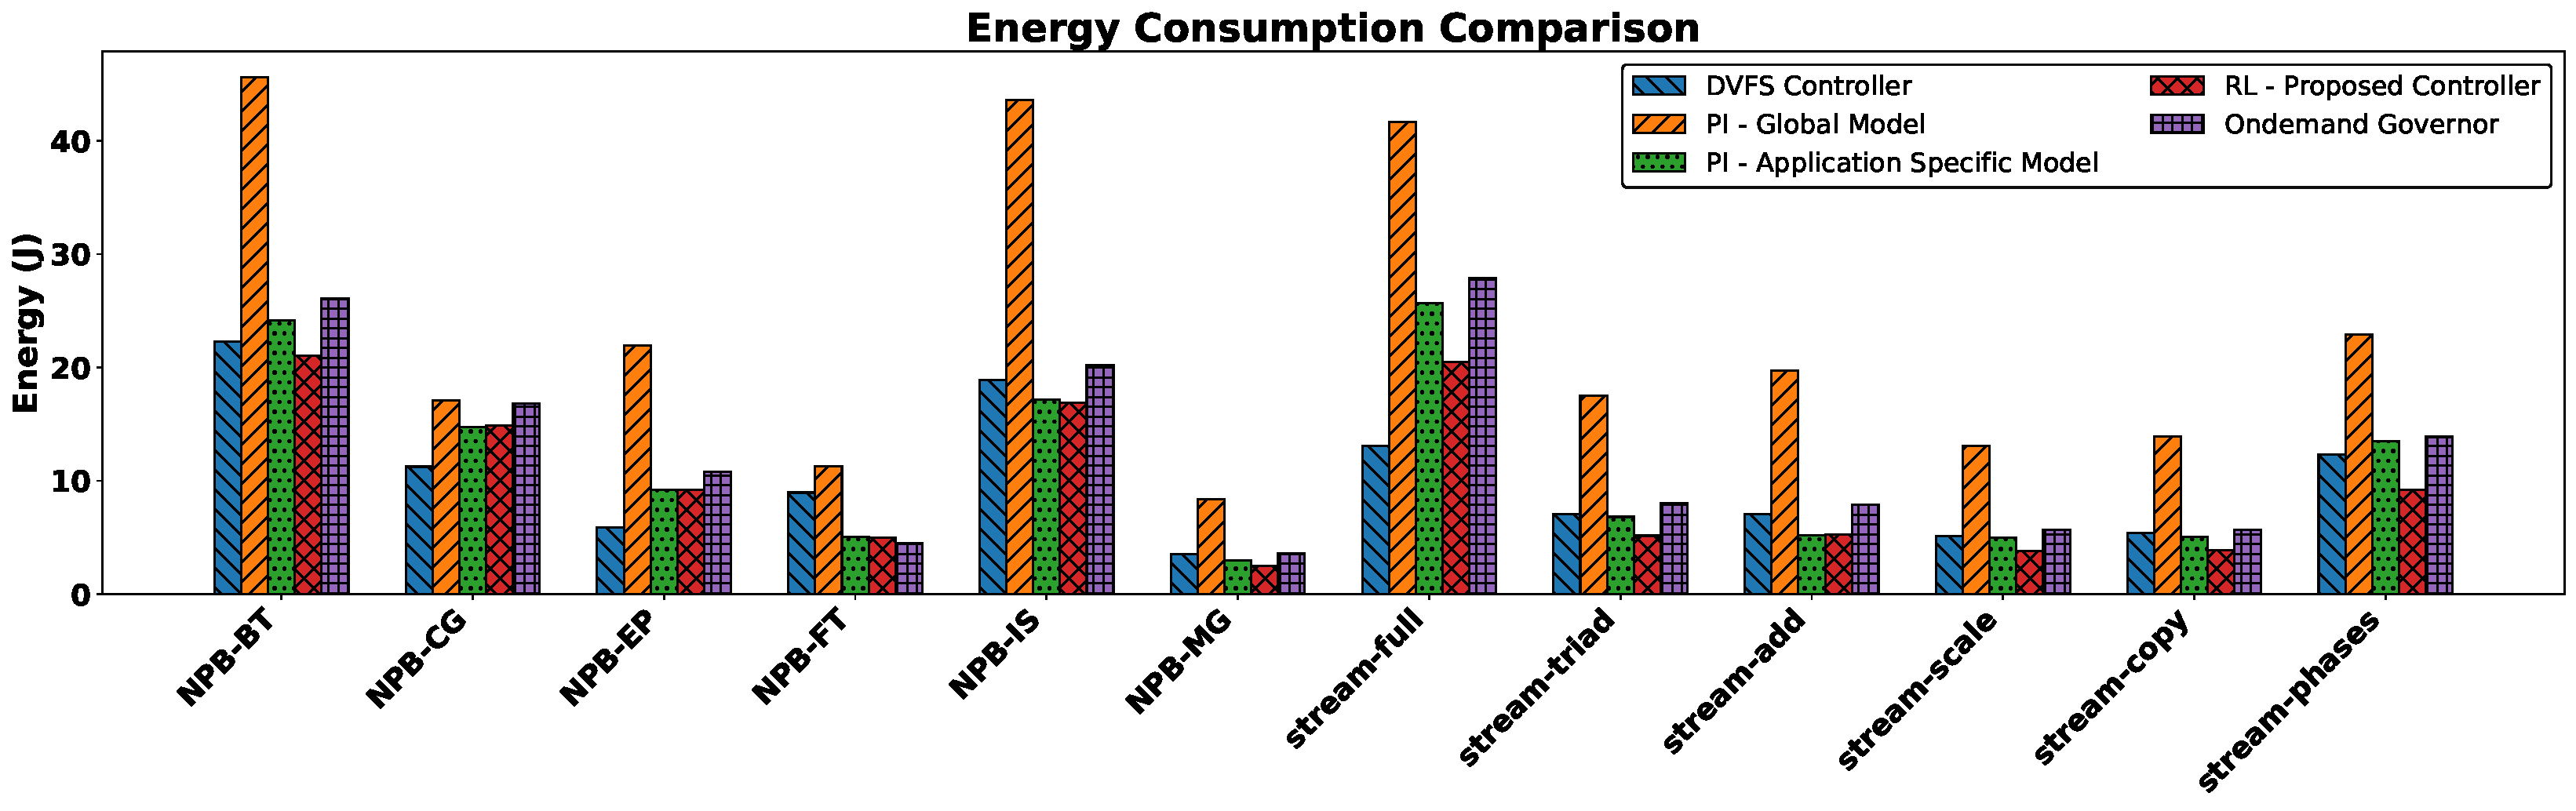
\includegraphics[width=\textwidth]{Figures/energy_consumption_comparison_with_dvfs_ondemand.pdf}
        \caption*{}
        \label{fig:PI-controller}
    \end{subfigure}\hfill
    \vspace{-0.5cm}
    \begin{subfigure}[b]{0.48\textwidth}
        \centering   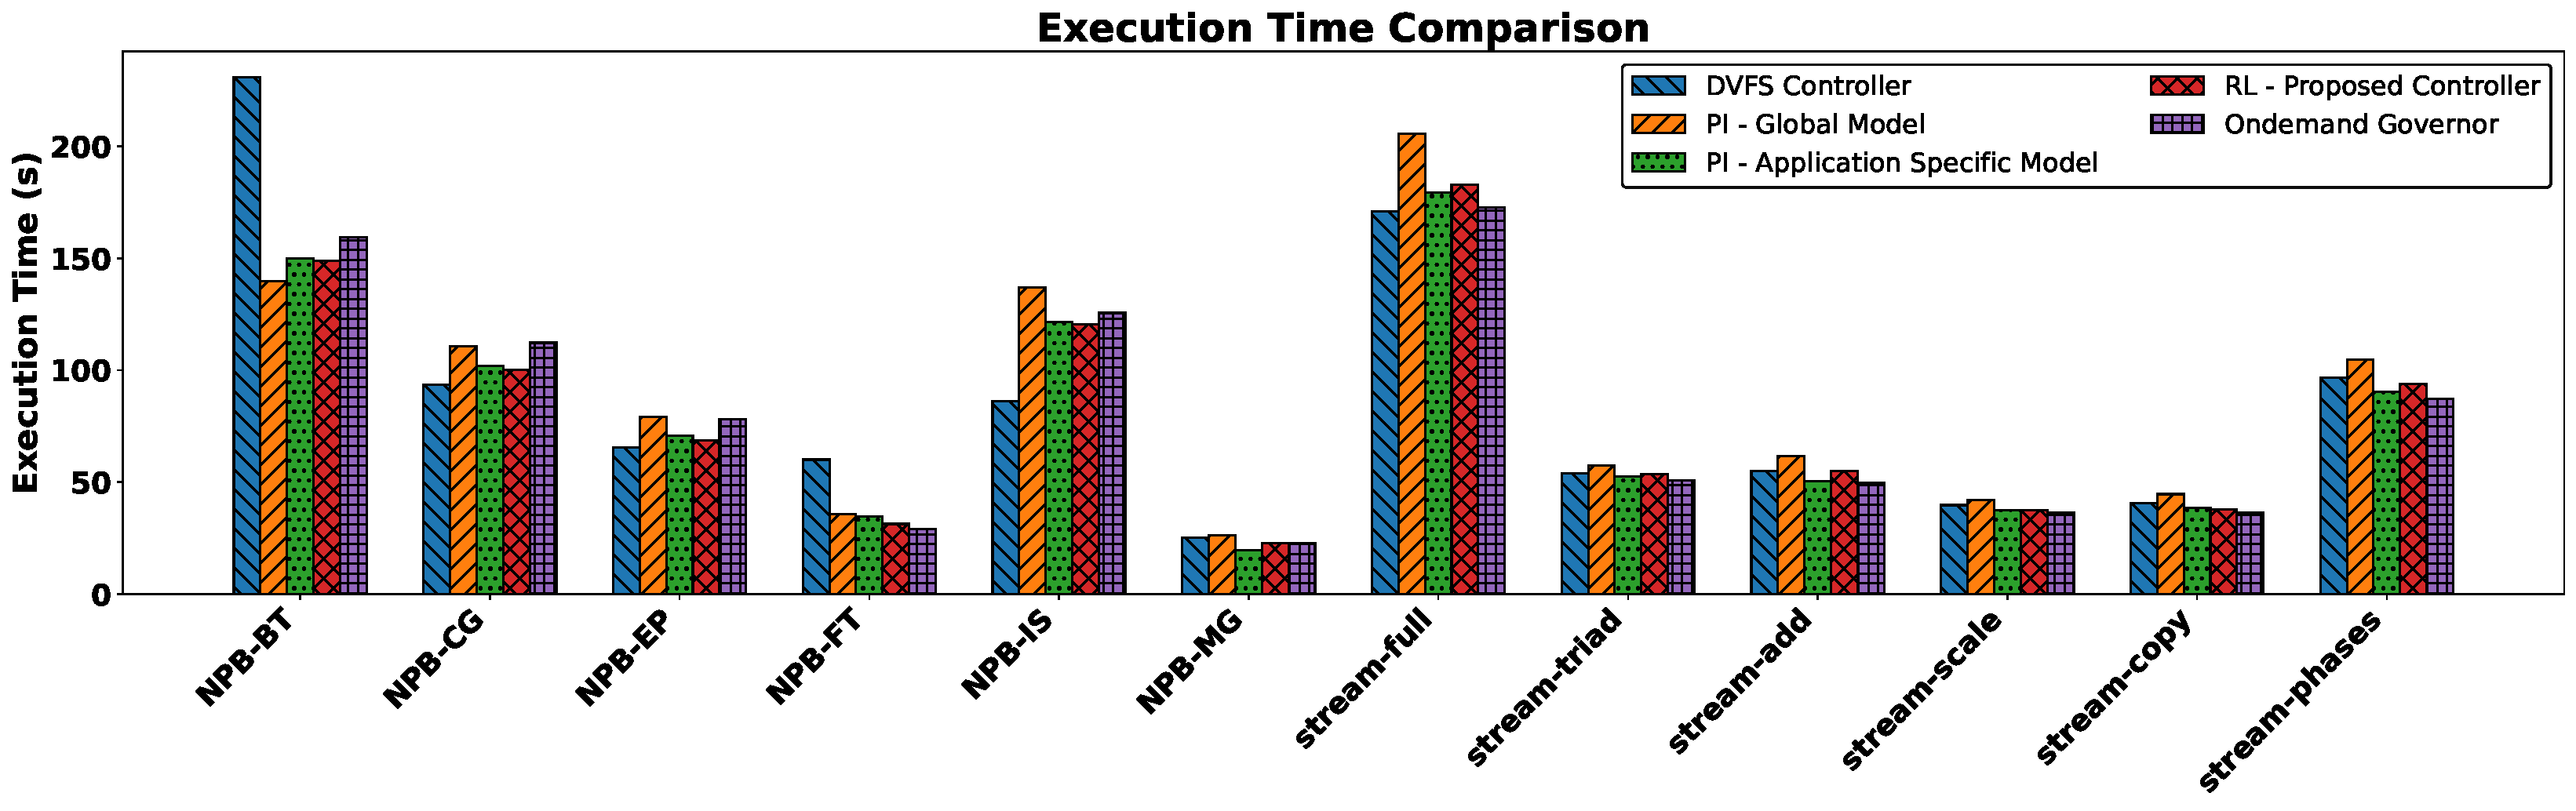
\includegraphics[width=\textwidth]{Figures/execution_time_comparison_with_dvfs_ondemand.pdf}
        \caption*{}
        \label{fig:RL-controller}
    \end{subfigure}
    % \vspace{-0.5cm}
    \caption{\small{Aggregate comparison between the proposed RL-based power-capping controller and four baselines: global PI, application-specific PI, DVFS, and the \textit{ondemand} governor.}
    % The RL controller achieves average energy savings of 59.19\% (vs. Global PI), 12.75\% (vs. App-Specific PI), 6.38\% (vs. DVFS Controller), and 23.09\% (vs. \textit{Ondemand} Governor), with corresponding average performance differences of –9.91\%, 1.22\%, –4.24\%, and 0.81\%, respectively.
    }
    \label{fig:comparison_PI}
%    \Description{Motivating example}
\end{figure}



% \sisetup{
%   scientific-notation=true,
%   round-mode=figures,
%   round-precision=3,
%   detect-weight=true,          
%   detect-inline-weight=math   
% }
% \newcommand{\bestg}[1]{\cellcolor{green!25}\textbf{#1}}
% \newcommand{\worstr}[1]{\cellcolor{red!15}#1}

% \begin{table*}[t]
% \begin{center}
% \resizebox{\textwidth}{!}{%
% \begin{tabular}{|c|ccc|ccc|ccc|ccc|ccc|}
% \hline
% \multirow{3}{*}{\textbf{Benchmark}} &
% \multicolumn{3}{c|}{\textbf{DVFS Controller}} &
% \multicolumn{3}{c|}{\textbf{PI-Global Model}} &
% \multicolumn{3}{c|}{\textbf{PI-App-Specific Model}} &
% \multicolumn{3}{c|}{\textbf{Ondemand Governor}} &
% \multicolumn{3}{c|}{\textbf{RL (Ours)}} \\
% \cline{2-16}
% & \shortstack{\scriptsize Energy\\Saved (\%)} & \shortstack{\scriptsize Perf\\Degrad. (\%)} & \textbf{ED$^{2}$P} &
%   \shortstack{\scriptsize Energy\\Saved (\%)} & \shortstack{\scriptsize Perf\\Degrad. (\%)} & \textbf{ED$^{2}$P} &
%   \shortstack{\scriptsize Energy\\Saved (\%)} & \shortstack{\scriptsize Perf\\Degrad. (\%)} & \textbf{ED$^{2}$P} &
%   \shortstack{\scriptsize Energy\\Saved (\%)} & \shortstack{\scriptsize Perf\\Degrad. (\%)} & \textbf{ED$^{2}$P} &
%   \shortstack{\scriptsize Energy\\Saved (\%)} & \shortstack{\scriptsize Perf\\Degrad. (\%)} & \textbf{ED$^{2}$P} \\
% \cline{2-16}
% &  &  &  &  &  &  &  &  &  &  &  &  &  &  &  \\
% \hline
% \textbf{NPB-BT} &
% 3.08 & \worstr{64.91} & \worstr{\num{1.18772e6}} &
% \worstr{-98.43} & \bestg{-0.21} & \num{8.90421e5} &
% -5.12 & 7.14 & \num{5.43782e5} &
% -13.50 & 13.90 & \num{6.63436e5} &
% \bestg{8.34} & 6.43 & \bestg{\num{4.67824e5}} \\
% \hline

% \textbf{NPB-CG} &
% \bestg{25.42} & \bestg{-7.38} & \bestg{\num{9.84159e4}} &
% \worstr{-13.56} & 9.57 & \num{2.09714e5} &
% 2.23 & 0.99 & \num{1.53389e5} &
% -11.47 & \worstr{11.17} & \worstr{\num{2.11919e5}} &
% 1.37 & -0.83 & \num{1.49226e5} \\
% \hline

% \textbf{NPB-EP} &
% \bestg{40.02} & \bestg{-3.04} & \bestg{\num{2.53050e4}} &
% \worstr{-124.00} & \worstr{16.87} & \worstr{\num{1.37298e5}} &
% 6.33 & 4.43 & \num{4.58408e4} &
% -9.97 & 15.63 & \num{6.59907e4} &
% 5.93 & 1.47 & \num{4.34663e4} \\
% \hline

% \textbf{NPB-FT} &
% \worstr{-77.46} & \worstr{96.27} & \worstr{\num{3.23267e4}} &
% -123.59 & 16.31 & \num{1.43021e4} &
% 0.02 & 13.07 & \num{6.04468e3} &
% \bestg{10.51} & \bestg{-5.16} & \bestg{\num{3.80638e3}} &
% 1.78 & 2.40 & \num{4.86997e3} \\
% \hline

% \textbf{NPB-IS} &
% 1.52 & \bestg{-26.02} & \bestg{\num{1.40667e5}} &
% \worstr{-127.69} & \worstr{17.41} & \worstr{\num{8.18978e5}} &
% 10.45 & 4.28 & \num{2.54109e5} &
% -5.54 & 7.65 & \num{3.19145e5} &
% \bestg{11.96} & 3.43 & \num{2.45745e5} \\
% \hline

% \textbf{NPB-MG} &
% -11.04 & 27.19 & \num{2.23950e3} &
% \worstr{-162.41} & \worstr{33.39} & \worstr{\num{5.82111e3}} &
% 6.23 & \bestg{-1.32} & \bestg{\num{1.13841e3}} &
% -12.72 & 15.20 & \num{1.86513e3} &
% \bestg{21.79} & 14.48 & \num{1.27779e3} \\
% \hline

% \textbf{Stream-Full} &
% \bestg{53.74} & \bestg{-0.82} & \bestg{\num{3.82039e5}} &
% \worstr{-47.49} & \worstr{19.33} & \worstr{\num{1.76332e6}} &
% 9.21 & 4.06 & \num{8.25458e5} &
% 1.23 & 0.29 & \num{8.34002e5} &
% 27.50 & 6.19 & \num{6.86421e5} \\
% \hline

% \textbf{Stream-Triad} &
% 7.66 & 12.86 & \num{2.05003e4} &
% \worstr{-128.48} & \worstr{20.24} & \worstr{\num{5.75778e4}} &
% 11.17 & 10.48 & \num{1.88981e4} &
% -4.44 & \bestg{6.45} & \num{2.06296e4} &
% \bestg{32.82} & 12.58 & \bestg{\num{1.48407e4}} \\
% \hline

% \textbf{Stream-Add} &
% 10.97 & 13.96 & \num{2.14976e4} &
% \worstr{-147.56} & \worstr{27.35} & \worstr{\num{7.46519e4}} &
% \bestg{35.17} & \bestg{4.60} & \bestg{\num{1.31873e4}} &
% 0.60 & 2.87 & \num{1.95567e4} &
% 33.77 & 13.80 & \num{1.59476e4} \\
% \hline

% \textbf{Stream-Scale} &
% 9.61 & 15.77 & \num{8.06690e3} &
% \worstr{-131.15} & \worstr{22.24} & \worstr{\num{2.29990e4}} &
% 12.17 & 8.75 & \num{6.91671e3} &
% -0.84 & \bestg{6.49} & \num{7.61543e3} &
% \bestg{32.65} & 8.75 & \bestg{\num{5.30353e3}} \\
% \hline

% \textbf{Stream-Copy} &
% 5.63 & 16.86 & \num{8.86046e3} &
% \worstr{-143.02} & \worstr{28.76} & \worstr{\num{2.77001e4}} &
% 11.65 & 11.53 & \num{7.55612e3} &
% 1.23 & \bestg{4.82} & \num{7.46148e3} &
% \bestg{32.83} & 8.64 & \bestg{\num{5.45115e3}} \\
% \hline

% \textbf{Stream-Phases} &
% 11.15 & 14.51 & \num{1.14581e5} &
% \worstr{-65.80} & \worstr{24.02} & \worstr{\num{2.50832e5}} &
% 2.20 & 7.12 & \num{1.10376e5} &
% -0.35 & \bestg{3.38} & \num{1.05472e5} &
% \bestg{33.35} & 11.47 & \bestg{\num{8.14447e4}} \\
% \hline\hline

% \textbf{Average} &
% 8.69 & 18.76 & \num{1.70185e5} &
% \worstr{-109.43} & \worstr{19.61} & \worstr{\num{3.56135e5}} &
% 8.48 & 6.26 & \num{1.65558e5} &
% -3.77 & 6.89 & \num{1.88408e5} &
% \bestg{20.34} & \bestg{7.40} & \bestg{\num{1.43485e5}} \\
% \hline
% \end{tabular}
% }
% \caption{Controllers compared to uncapped (Max PCAP). Only row-wise extremes are colored: \textbf{green} = best (max Energy Saved, min Perf Degradation, min ED$^{2}$P); \textbf{red} = worst (min Energy Saved, max Perf Degradation, max ED$^{2}$P). Lower ED$^{2}$P is better.}
% \label{tab:controllers_vs_uncapped_extremes}
% \end{center}
% \end{table*}







% Figure \ref{fig:phases_timeline} outlines the application's progress, measured power, and $PCAP$ during the runtime under both uncapped and controlled settings. When analyzing the uncapped execution of the $PHASES-STREAM-FULL$ application, we noted a variable performance across two distinct levels while energy consumption remained relatively unchanged. In contrast, the RL controller, tuned itself to the characteristics of each kernel, modulated the $PCAP$ to an optimal average level bringing down the performance negligibly. This dynamic regulation of power is evident not only in the stepped $PCAP$ output generated by the controller but also in the $progress$ values across the application's four phases, each linked to a specific kernel.

% Next, for evaluating the efficiency of the controller to varying performance scenarios, it is important to test the controller while running an application with varying phases. 
% We evaluate the ability of the proposed controller to adapt to varying phases of the application during the runtime by testing it on a $STREAM$ application running different kernels iteratively. We chose the $STREAM$ full application with all four kernels being executed $1000$ times for a cycle of $10$ iterations repeatedly. Initially we execute the application without any $PCAP$ (uncapped), ensuring maximum power delivered to the CPU cores. We then run the application under the supervision of the proposed controller and compared the energies consumed and their corresponding execution times. It was observed that the uncapped system consumed $290.380 \unit{\kilo \joule}$ of energy for an execution time of $1773.99 \unit{\second}$, while the controlled run costed only $210.444 \unit{\kilo \joule}$ of energy, for a runtime of $1925 \unit{\second}$. The statistics show a reduction of only $8.5 \%$ of performance, while saving $27.5\%$ energy. This in-fact verifies the ability of the controller to adapt to dynamic environments. Figure \ref{fig:phases_timeline} shows the $progress$, measured power $power$ and $PCAP$ during the run-time of the STREAM application with phases, under uncapped and controlled environments. The uncapped runs of $phases-stream-full$ application shows varying performance of two levels, under nearly constant energy consumption. On the other-hand, RL controller, observing the kernel properties regulated the $PCAP$ at minimum average value that gives the maximum performance in return.  This dynamics in the regulation of average power can be observed not only from the layered $PCAP$ (controller output), but also from the progress reports split over four phases, corresponding to four different kernels of the application.

% \begin{figure}[htb]
%         \centering
%         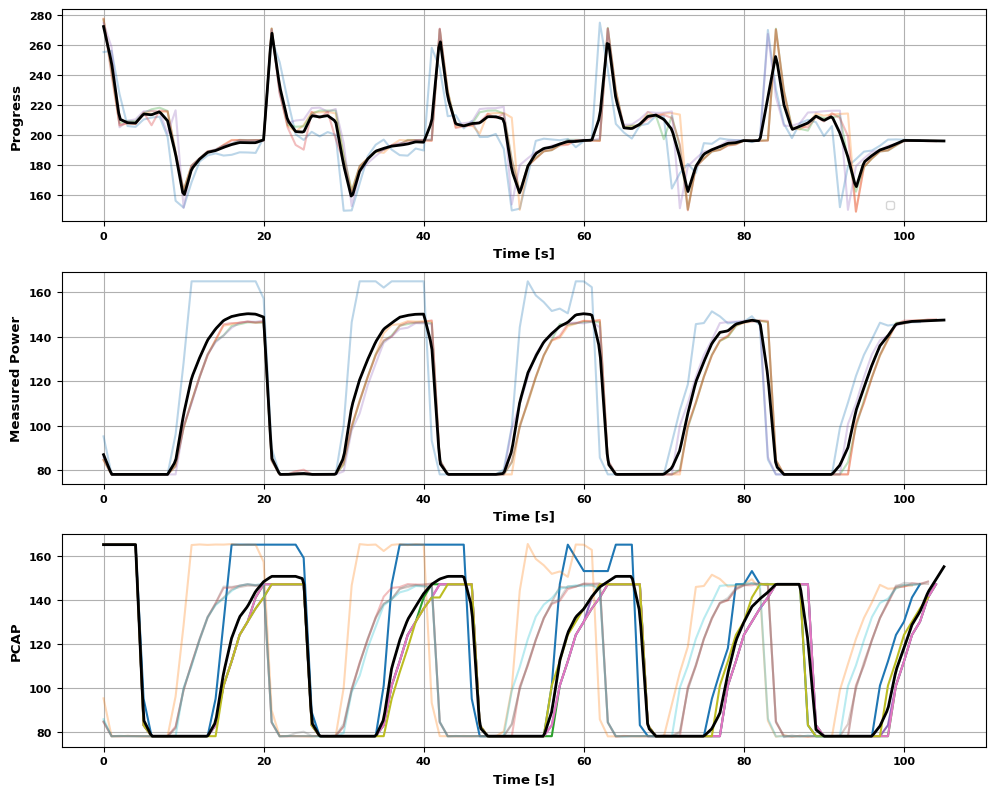
\includegraphics[width=\columnwidth]{Figures/PI_controller.png} % first figure itself
%         \caption{\small{Time series plot of a single execution of $phases-stream-full$ application with phases showing a) progress, b) Measured Power and c) PCAP values under proposed controller (orange) and uncapped power.}}
%         \Description{Application with phases}
%         \label{fig:phases_timeline}
% \end{figure}


% To underscore the controller's capacity to adjust to unfamiliar runtime environments, we assessed its performance with more applications not previously encountered during its training. The testing applications consists both memory-intensive and compute intensive benchmarks. Figure \ref{fig:comparison} presents these application's performance under both controlled and uncontrolled conditions. As expected the performance decreased due to the controller's tuning for maximum efficiency but maintained it at lower EDP regions.

% This time the $ONES-NPB-IS$ application, was configured with a problem size of 26 and was run for 10000 iterations. In an uncapped environment, the application completed in $1169.1 \unit{\second}$, using $187.22 \unit{\kilo \joule}$ of energy. In contrast, when managed by the controller, the application finished in $1249.2 \unit{\second}$ and used $167.7 \unit{\kilo \joule}$ of energy - a slight performance decay of approximately 6.84\% but with an energy savings of 10.42\%. The consistency and efficiency of the controller in managing the ones-npb-is runs were previously detailed while reviewing the repeatability results in Figure \ref{fig:comparison} and are further supported by the data in Table \ref{tab:repeatability}.


% To further emphasize the ability of the controller to adapt to new runtime environments, we evaluate the controller with a new application which it has never encountered during the training phase. This application, $ones-npb-is$ is a memory bound application. Figure \ref{fig:npb_is_timeline} shows the results depicting the runtime performance of the application under controlled and uncontrolled scenarios.  It is important to note that there is a drop in the performance on account of adjusting to the maximum efficiency point. The $npb-is$ application was executed for $10000$ iterations under a problem size of $26$. It was executed in $1156 \unit{\second}$ in an uncapped environment while consuming $187.22 \unit{\kilo \joule}$ of energy, whereas under the proposed controller, a run time of $1290 \unit{\second}$ and an energy consumption of $167.7 \unit{\kilo \joule}$ of energy was recorded. The efficiency of the controller during the repeated runs of $ones-npb-is$, has already been discussed while explaining the repeatability statistics in Figure \ref{fig:comparison} with the help of Table \ref{tab:repeatability}.



% \begin{figure}[htb]
%         \centering
%         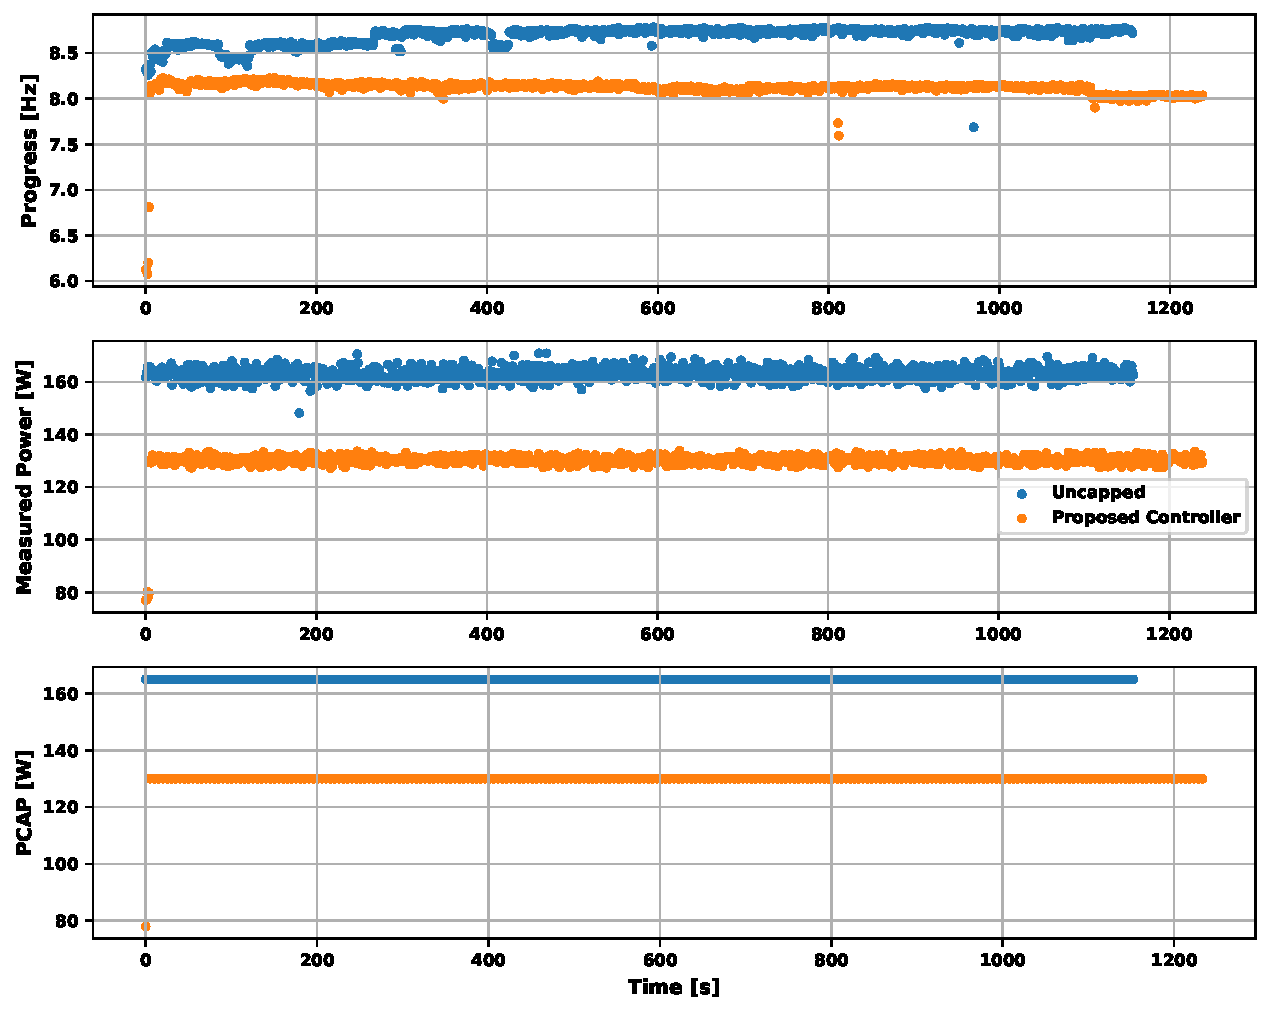
\includegraphics[width=\columnwidth]{Figures/ones-npb-is.pdf} % first figure itself
%         \caption{\small{Time series plot of a single execution of $npb-is$, a new test application showing a) progress, b) Measured Power and c) PCAP values for controlled and uncapped cases.}}
%     \label{fig:npb_is_timeline}
%     \Description{Application with phases}
% \end{figure}

%As an additional comment, it is important to note that the variance of the experiments under the proposed $RL$ controller, is less compared to the uncapped and minimum $PCAP$ runtime environments. This observation shows the presence of measurement noise that comes with overuse and under-use of node power caps. Increasing CPU power also leads to a rise in CPU cycles, which can be wasted if the hardware lacks adequate memory bandwidth, consequently leading to higher power consumption and overheating of components, without any corresponding boost in performance.


% The point shown in the red in the performance (execution time) vs power plots for each of these applications, corresponds to the run under the supervision of proposed controller. The remaining points corresponds to the runs of the applications under same problem size and iterations, under respective the power caps given by the legend. It can be seen that the RL controller was able regulate the power of each of these nodes under the maximum efficiency region of the node-application architecture, which means that the ratio of the energy saved to the performance compromised is at maximum while using the proposed controller. The Energy Delay Product ($EDP$) is a metric that measures how efficiently a system uses energy to perform a task. It is calculated by multiplying the amount of energy used by the time it takes to complete the task. 

% When the performance changes the power caps were changed ensuring that a minimum decay of performance only happened. It can be observed from the total change in the average progress value of \textcolor{red}{$20$} while the average power was reduced by \textcolor{red}{60W} during every cycle. This shows the ability of the controller to adapt to the varying performance and applications.



% \todo{remove mention of variability here, and add a note that the final version of the paper will include variability results too.}
% We next compare the variability and reproducibility statistics associated with the controller. Here we compare the proposed controller against the maximum and minimum power capped performance of an application on same hardware as well as different hardware multiple times and record the statistics. It is important to prove the stability and variability of the proposed controller under the same and different architectures. For reproducibility or stability test we reserve a node and run the phased application 10 times and record the observations. Figure \ref{fig:comparison} also shows the run time performance statistics with mean of their execution times and consumed energy values. Table \ref{tab:repeatability} depicts the corresponding statistics.
